%%%%%%%%%%%%%%%%%%%%%%%%%%%%%%%%%%%%%%%%%%%%%%%%%%%%%%%%%%%%%%%%%%%%%%%%%%%%%%%%
% Thesis / Project Report
% LaTeX Template
% Version 2.0 (08/04/16)
%
% Author:
% Siddhant Shrivastava
% https://github.com/sidcode/bits-pilani-thesis-template-latex
%
% This template is heavily based on the work of Darshit Shah, Steven Gunn and Sunil Patel
% Darshit Shah
% https://github.com/darnir/BPHC-LaTeX-Report-Class
% Steven Gunn
% http://users.ecs.soton.ac.uk/srg/softwaretools/document/templates/
% and
% Sunil Patel
% http://www.sunilpatel.co.uk/thesis-template/
%
% License:
% CC BY-NC-SA 4.0 (http://creativecommons.org/licenses/by-nc-sa/4.0/)
%
% Note:
% Make sure to edit document variables in the Thesis.cls file
%
%%%%%%%%%%%%%%%%%%%%%%%%%%%%%%%%%%%%%%%%%%%%%%%%%%%%%%%%%%%%%%%%%%%%%%%%%%%%%%%%

%-------------------------------------------------------------------------------
%	PACKAGES AND OTHER DOCUMENT CONFIGURATIONS
%-------------------------------------------------------------------------------

\documentclass[11pt, a4paper, oneside]{Thesis} % Paper size, default font size
                                               % and one-sided paper

\graphicspath{{Pictures/}} % Specifies the directory where pictures are stored

\usepackage[backend=bibtex]{biblatex}
\usepackage{bm}
\bibliography{Bibliography.bib}

\title{\ttitle} % Defines the thesis title - don't touch this

\begin{document}

\frontmatter % Use roman numbering style (i, ii...) for the pre-content pages

\setstretch{1.3} % Line spacing of 1.3

% Define page headers using FancyHdr package and set up for one-sided printing
\fancyhead{} % Clears all page headers and footers
\rhead{\thepage} % Sets the right side header to show the page number
\lhead{} % Clears the left side page header

\pagestyle{fancy} % Finally, use the "fancy" page style to implement the
                  %FancyHdr headers

% Input all the variables used in the document. Please fill out the
% variables.tex file with all your details.
%-------------------------------------------------------------------------------
%	DOCUMENT VARIABLES
%
%	Fill in the lines below to set the various variables for the document
%-------------------------------------------------------------------------------

%-------------------------------------------------------------------------------
% Your thesis title - this is used in the title and abstract
% Command: \ttitle
\thesistitle{Chaos and its Applications}
%-------------------------------------------------------------------------------
% The document type: Thesis / report, etc.
% Command: \doctype
\documenttype{Undergraduate Thesis Mid Semester Report}
%-------------------------------------------------------------------------------
% Your supervisor's name - this is used in the title page
% Command: \supname
\supervisor{Dr. Pallab \textsc{Basu}}
%-------------------------------------------------------------------------------
% The supervisor's position - Used on Certificate
% Command: \suppos
\supervisorposition{Faculty}
%-------------------------------------------------------------------------------
% Supervisor's institute
% Command: \supinst
\supervisorinstitute{International Centre for Theoretical Sciences, Bangalore}
%-------------------------------------------------------------------------------
% Your Co-Supervisor's name
% Command: \cosupname
%\cosupervisor{Dr. FirstName \textsc{SecondName}}
%-------------------------------------------------------------------------------
% Co-Supervisor's Position - Used on Certificate
% Command: \cosuppos
%\cosupervisorposition{Asst. Professor}
%-------------------------------------------------------------------------------
% Co-Supervisor's Institute
% Command: \cosupinst
%\cosupervisorinstitute{BITS-Pilani Hyderabad Campus}
%-------------------------------------------------------------------------------
% Your Examiner's name. Not currently used anywhere.
% Command: \examname
\examiner{}
%-------------------------------------------------------------------------------
% Name of your degree
% Command: \degreename
\degree{Bachelor of Engineering (Hons.)}
%-------------------------------------------------------------------------------
% The BITS Course Code for which this report is written
% COmmand: \ccode
\coursecode{BITS F422T}
%-------------------------------------------------------------------------------
% The name of the Course
% Command: \cname
\coursename{Thesis}
%-------------------------------------------------------------------------------
% Your name. Extend manually in case of multiple authors
% Command: \authornames
\authors{Aditya \textsc{Vijaykumar}}
%-------------------------------------------------------------------------------
% Your ID Number - used on the Title page and abstract
% Command: \idnum
\IDNumber{2013B5A4688P}
%-------------------------------------------------------------------------------
% Your address
% Command: \addressnames
\addresses{}
%-------------------------------------------------------------------------------
% Your subject area
% Command: \subjectname
\subject{}
%-------------------------------------------------------------------------------
% Keywords for this report.
% Command: \keywordnames
\keywords{}
%-------------------------------------------------------------------------------
% University details
% Command: \univname
\university{\texorpdfstring{\href{http://www.bits-pilani.ac.in/} % URL
                {Birla Institute of Technology and Science Pilani}} % University name
                {Birla Institute of Technology and Science Pilani}}
%-------------------------------------------------------------------------------
% University details, in Capitals
% Command: \UNIVNAME
\UNIVERSITY{\texorpdfstring{\href{http://www.bits-pilani.ac.in/} % URL
                {BIRLA INSTITUTE OF TECHNOLOGY AND SCIENCE PILANI}} % name in capitals
                {BIRLA INSTITUTE OF TECHNOLOGY AND SCIENCE PILANI}}

%-------------------------------------------------------------------------------
% Campus Name
% Command: \campusname
\campus{Pilani Campus}

%-------------------------------------------------------------------------------
% Campus Name, in capitals
% Command: \CAMPUSNAME
\CAMPUS{PILANI CAMPUS}


%-------------------------------------------------------------------------------
% Department Details
% Command: \deptname
\department{\texorpdfstring{\href{http://www.bits-pilani.ac.in/pilani/computerscience/ComputerScience} % Your department's URL
                {Computer Science \& Information Systems}} % Your department's name
                {Computer Science}}
%-------------------------------------------------------------------------------
% Department details, in Capitals
% Command: \DEPTNAME
\DEPARTMENT{\texorpdfstring{\href{http://www.bits-pilani.ac.in/pilani/computerscience/ComputerScience} % Your department's URL
                {COMPUTER SCIENCE \& INFORMATION SYSTEMS}} % Your department's name in capitals
                {COMPUTER SCIENCE \& INFORMATION SYSTEMS}}
%-------------------------------------------------------------------------------
% Research Group Details
% Command: \groupname
\group{\texorpdfstring{\href{Research Group Web Site URL Here (include http://)}
                {Research Group Name}} % Your research group's name
                {Research Group Name}}
%-------------------------------------------------------------------------------
% Research Group Details, in Capitals
% Command: \GROUPNAME
\GROUP{\texorpdfstring{\href{Research Group Web Site URL Here (include http://)}
                {RESEARCH GROUP NAME (IN BLOCK CAPITALS)}}
                {RESEARCH GROUP NAME (IN BLOCK CAPITALS)}}
%-------------------------------------------------------------------------------
% Faculty details
% Command: \facname
\faculty{\texorpdfstring{\href{Faculty Web Site URL Here (include http://)}
                {Faculty Name}}
                {Faculty Name}}
%-------------------------------------------------------------------------------
% Faculty details, in Capitals
% Command: \FACNAME
\FACULTY{\texorpdfstring{\href{Faculty Web Site URL Here (include http://)}
                {FACULTY NAME (IN BLOCK CAPITALS)}}
                {FACULTY NAME (IN BLOCK CAPITALS)}}
%-------------------------------------------------------------------------------


%-------------------------------------------------------------------------------
%   NON-CONTENT PAGES
%-------------------------------------------------------------------------------
\maketitle
%\Declaration
%\Certificate
%\Quotation{Insert Random Quote here. Publish like a boss.}{Your Name}

%-------------------------------------------------------------------------------
%	LIST OF CONTENTS/FIGURES/TABLES PAGES
%-------------------------------------------------------------------------------

% The page style headers have been "empty" all this time, now use the "fancy"
% headers as defined before to bring them back
\pagestyle{fancy}

\lhead{\emph{Contents}} % Set the left side page header to "Contents"
\tableofcontents % Write out the Table of Contents

% Set the left side page header to "List of Figures"
\lhead{\emph{List of Figures}}
%\listoffigures % Write out the List of Figures

 % Set the left side page header to "List of Tables"
\lhead{\emph{List of Tables}}
%\listoftables % Write out the List of Tables

%-------------------------------------------------------------------------------
%	SYMBOLS
%-------------------------------------------------------------------------------

\clearpage % Start a new page

\lhead{\emph{Glossary}} % Set the left side page header to "Symbols"

%\listofnomenclature % List the nomenclature. (We use the glossaries package)

%-------------------------------------------------------------------------------
%	DEDICATION
%-------------------------------------------------------------------------------

\setstretch{1.3} % Return the line spacing back to 1.3

\pagestyle{empty} % Page style needs to be empty for this page

% Dedication text
%\Dedicatory{Dedicate this to someone, anyone.}

\addtocontents{toc}{\vspace{2em}} % Add a gap in the Contents, for aesthetics

%-------------------------------------------------------------------------------
%	THESIS CONTENT - CHAPTERS
%-------------------------------------------------------------------------------

\mainmatter % Begin numeric (1,2,3...) page numbering

\pagestyle{fancy} % Return the page headers back to the "fancy" style

% Include the chapters of the thesis as separate files from the Chapters folder
% Uncomment the lines as you write the chapters

% Chapter 1

\chapter{Introduction} % Main chapter title

\label{Chapter1} % For referencing the chapter elsewhere, use \ref{Chapter1} 

\lhead{Chapter 1. \emph{Introduction}} % This is for the header on each page - perhaps a shortened title

%----------------------------------------------------------------------------------------
It is a triumph of physics and its practitioners that we can reproduce the dynamics of extremely complex systems using mathematical equations. The problem, however, is that most of the governing equations of these complex systems are highly nonlinear, and often coupled differential equations. This makes it very difficult for us to solve the systems in question exactly, 

But this was not entirely unexpected. It is easy to notice that most systems that we come across in day-to-day life are not simple systems. Something as basic as the simple pendulum does not follow $\ddot{\theta} + \omega^2\theta = 0$ if $\theta$ is large (higher order corrections to $\theta$ starts dominating). This tells us that even the most basic of the systems have to be nonlinear.

In-principle, the state of a system at present is completely determined by initial conditions. Such systems are called \textit{deterministic system}. So for different initial conditions, we could have trajectories that diverge exponentially faster from each other in time. Such systems are said to be \textit{chaotic systems}. Let's say $\delta x$ be the separation between two trajectories. We can then give a rough mathematical definition of complexity as follows
$$\delta x(t) = \exp{\lambda t} \ \delta x(0)$$
The $\lambda$ in the exponent is called the \textit{Lyapunov exponent}. This quantifies the speed at which the systems moves towards chaos - a higher $\lambda$ means that the system will go to chaos faster.

In this thesis, we shall explore different aspects of chaos in different physical systems. Broadly, we shall divide the systems that we'll consider into \textit{classical} and \textit{quantum} systems. We shall consider some specific cases in each of these, and get into the depth of it.

\newpage

\section{Outline and Description}
We give a brief outline description of each of the cases that we are going to consider in this thesis :-
\begin{itemize}
	\item \textbf{Settting up the Machinery} - we shall set up the basic analytic and numerical machinery used for calculating various quantities in chaotic systems. We shall first review a bit of Hamiltonian dynamics, and then look into mappings, Poincare sections, and also go into detail as to how one describes the stability of points and trajectories. We shall also see how we can use symbolic algebra and numerical softwares to get an idea of the dynamics of chaotic systems.
	
	\item \textbf{The Logistic Map} - The Logistic Map is a simple map of degree two, which is astoundingly effective while studying population dynamics and epidemic growth. It also holds immense interest from a mathematical point of view and will also be a useful tool when we discuss some aspects of chaos in quantum systems. We write down the logistic map and derive the stable points of the systems. We see that the system inherently gives rise to a \textit{bifurcation diagram} in phase space, which will show clear signatures of chaotic dynamics.
	
	\item \textbf{Lorenz System of Differential Equations and the Lorenz Attractor} - The Lorenz system is probably the most well illustrated system of deterministic chaos. It was initially written down to describe the dynamics of convective atmosphere currents, but has found applications in other fields as well. We shall start with defining the system, and doing an analysis of the form of the equations, the parameters involved, and a stability analysis. We shall then evaluate the system numerically and show that it indeed is chaotic.
	
	\item \textbf{Miscellaneous Systems in Classical Chaos} - We shall define a few systems of our own, and try to study their classical chaotic dynamics using numerical methods.
	
	\item \textbf{Quantum Chaos} - We look at how chaos arises in quantum system, and investigate the link between a classically chaotic system and the quantum spectrum of the system.
	
	\item \textbf{A Bound on Chaos} - We study the conjecture by Maldacena, Stanford and Shenker \cite{Maldacena:2015waa} which gives an upper limit to how fast chaos can grown in a quantum chaotic system. We see that this bound is exactly satisfied for black holes.
	
	\item \textbf{Chaos in Quantum Channels} - We study the growth of chaos in a quantum information perspective \cite{Hosur:2015ylk}, and try to define an independent information theoretic definition of chaos, referring to 
	
\end{itemize}



% Chapter Template

\chapter{Setting up the Machinery} % Main chapter title

\label{ChapterX} % Change X to a consecutive number; for referencing this chapter elsewhere, use \ref{ChapterX}

\lhead{Chapter 2. \emph{Setting up the Machinery}} % Change X to a consecutive number; this is for the header on each page - perhaps a shortened title

Since this chapter is mostly a review, we have borrowed from \cite{strogatz_2015}, \cite{tabor_1989} and \cite{ott_2008} 
\section{Hamiltonian Dynamics}
Given a Hamiltonian $H(q,p)$, one can write down Hamilton's equations of motion as follows

$$\dot{q_i} = \frac{\partial H}{\partial p_i}, \ \dot{p_i} = -\frac{\partial H}{\partial q_i} $$

Here, $q_i$ and $p_i$ are said to be phase space coordinates, and $x=(q,p)$ with $q=(q_1,q_2,\ldots,q_N)$ and $p=(p_1,p_2,\ldots,P_N)$ is said to be a point in phase space. We can see that Hamilton's equation indeed gives the path in time of the dynamical system in the phase space. One can write Hamilton's equation in vector form as
$$\dot{x_i} = \omega_{ij} \frac{\partial H(x)}{\partial x_j}, \ \omega = \left(\begin{array}{cc} 0 & I\\ -I & 0 \end{array}\right)$$
where $I$ is the identity matrix in the applicable dimension.

Note that we have chosen $H$ only to be a function of $q$ and $p$. $q$ and $p$ are functions of time $t$, but in our construction, the Hamiltonian is independent of time. The explicit time-dependence of the Hamiltonian is an important check to see if the system is conservative or non-conservative. We can see this in the following way, by assuming $H$ to be a function of $t$ as well.
$$\frac{d}{dt}H(q,p,t)=\frac{\partial H}{\partial q}\dot{q} + \frac{\partial H}{\partial p}\dot{p} + \frac{\partial H}{\partial t}$$
If $H$ is not a function of $t$, the first two terms cancel, and hte third term goes to zero, which gives us the identity that $\frac{d}{dt}H(q,p,t)=0$. This means that the phase space trajectories lie of curves of constant energy $E$. Thus, for the specific case of single degree of freedom systems, we can say that the dynamical system described by $H$ is integrable.

\section{Canonical Transformations}
We have been used to interpreting $q$ and $p$ as position and momentum respectively, but it is important in chaotic dynamics to abandon this notion and think of it just as variables in the phase space. In principle, we can work with new variables which are functions of the old variables, provided that this change obeys Hamilton's equations. These new variables are called canoncical variables, and the corresponding transformations are called \textit{canonical transformations}.

Consider,
$$\tilde{q} = f(q,p,t), \ \tilde{p}=g(q,p,t)$$
Corresponding to this, one could write the equations of motion as,
$$\frac{d\tilde{q}}{dt} = \frac{\partial \tilde{H}}{\partial p}, \ \ \frac{d\tilde{p}}{dt}=-\frac{\partial \tilde{H}}{\partial q}$$
where $\tilde{H} = \tilde{H}(\tilde{q},\tilde{p},t)$ is the Hamiltonian of the systems under the transformation.

%Fixed Points
%Limit Cycles

% Chapter Template

\chapter{Lorenz System of Differential Equations and the Lorenz Attractor} % Main chapter title

\label{ChapterX} % Change X to a consecutive number; for referencing this chapter elsewhere, use \ref{ChapterX}

\lhead{Chapter 3. \emph{Lorenz System of Differential Equations and the Lorenz Attractor}} % Change X to a consecutive number; this is for the header on each page - perhaps a shortened title

The Lorenz system\cite{lorenz_1963} is described as follows :-
$$\dot{x} = \sigma(y-x)$$
$$\dot{y} = rx - y - xz$$
$$\dot{z} = xy - bz$$,
where $x,y,z$ are dynamical variables and $\sigma,r,b$ are constants.

These innocuous looking equations hold many secrets in them. The landmark 1963 paper by Lorenz describing these equations was written keeping in mind a convective model of atmospheric dynamics, but it has since found a wide variety of applications in lasers, circuits etc.

\section{A Few Properties}
\begin{itemize}
	\item Though the equations look simple, we can already see that the solutions might be complicated due to the nonlinearity in the terms $xy$ and $xz$. Nonlinear systems could lead to chaotic dynamics.
	\item One could try to solve these equations without much thought by putting it directly into a computer and getting a solution. But it is useful to note that the equation has a few symmetries. For example $(x,y,z) \rightarrow (-x,-y,z)$ keeps the solution invariant. This means that all solutions should be symmetric or have a redundant symmetric partner.
	\item One calls a system of equations dissipative if the phase space volume contracts as the system evolves in time. If we write the equations in a condensed form as $\dot{\boldsymbol{x}} = \boldsymbol{f}(\boldsymbol{x})$, then the volume the rate of change of volume is given by $\nabla.\boldsymbol{f}$ integrated over the volume. We can see
	$$\nabla.\boldsymbol{f} = \frac{\partial}{\partial x}[\sigma(y-x)] + \frac{\partial}{\partial y}[rx-y-xz] + \frac{\partial}{\partial z}[xy-bz] = -(\sigma +1 +b) < 0$$
	This is a negative constant. So, the phase space volume decreases in time and the Lorenz system is dissipative.
	\item Lets consider the Lorenz system without the nonlinearities. If one looks closely, this system is equivalent to linearizing the original system by considering perturbations around the origin. The equations would then read,
	\begin{eqnarray}
		\dot{x} = \sigma(y-x) \\
		\dot{y} = rx - y \\
		\dot{z} = - bz,
	\end{eqnarray}
	We can immediately see that the equation for $z$ is decoupled from the other two. Also, the $z$ solution decays exponentially as $t\rightarrow \infty$. The other two equations can be written as :-
	$$\left(\begin{array}{cc} \dot{x} \\\dot{y} \end{array}\right) = \left(\begin{array}{cc} -\sigma & \sigma \\\ r & -1 \end{array}\right) \left(\begin{array}{cc} x \\y \end{array}\right)$$
	The determinant $\Delta=-\sigma(1-r)$ and trace $\tau = -(\sigma+1)$. The system has a saddle point at $r>1$
\end{itemize}	
\section{Numerical Solution}
We have seen that a signature of chaos is that the trajectories diverge for a slight change in the initial conditions. As these equations are not really very straightforward to solve analytically, we solve it numerically using Python. We use initial conditions as $(1,1,1)$ and $(1.0000001,1,1)$, and plot the variation of $x,y,z$ with time $t$. 

Fig. [\ref{fig:dyvar_vs_t}] plots the numerically integrated equation for these slightly different initial conditions. We see that this system shows clear signs of chaos - the trajectories start diverging after $t=30$ or so. This is clearly evident from Fig. [\ref{fig:delta_trajectory}], which plots the deviation of paths from each other with time.

\begin{figure}[h!]
	\centering
	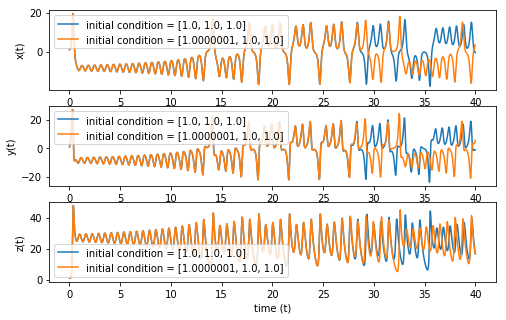
\includegraphics[scale=0.8]{Figures/dyvar_vs_t.png}
	\caption[An Electron]{Numerical solutions for different initial conditions. Trajectories start to visibly diverge roughly around $t=30$.}
	\label{fig:dyvar_vs_t}
\end{figure}

Typically, if we take the two initial conditions far away from each other, we will se that the system goes to chaos faster. This is in agreement with what we had expected and conjectured.

\begin{figure}[h!]
	\centering
	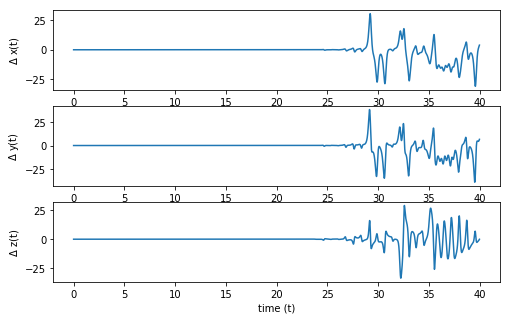
\includegraphics[scale=0.8]{Figures/delta_trajectory.png}
	\caption[An Electron]{The deviation of paths with start out very close to each other at tie $t=0$.}
	\label{fig:delta_trajectory}
\end{figure}
Fig. [\ref{fig:3d_trajectory}] shows a beautiful 3-D plot of the numerically integrated solution, which looks like the wings of a butterfly. Probably because of this, chaos is also sometimes referred to as the \textit{butterfly effect}.

Lorenz's model is so powerful that it continues to be studied till today. We shall investigate this further in the thesis, and hope to make some more comments in the final report.
\begin{figure}[h!]
	\centering
	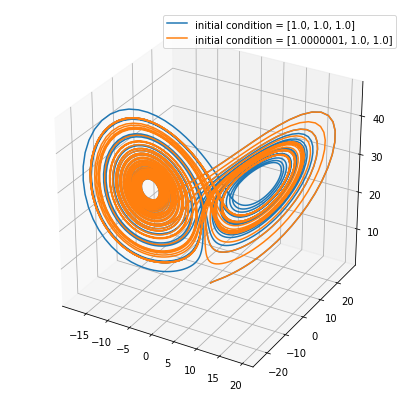
\includegraphics[scale=0.7]{Figures/3d_trajectory.png}
	\caption[An Electron]{A 3-D plot of $x,y,z$. Chaos is evident here too.}
	\label{fig:3d_trajectory}
\end{figure}

% Chapter Template

\chapter{The Logistic Map} % Main chapter title

\label{Chapter4} % Change X to a consecutive number; for referencing this chapter elsewhere, use \ref{ChapterX}

\lhead{Chapter 4. \emph{The Logistic Map}} % Change X to a consecutive number; this is for the header on each page - perhaps a shortened title
\section{The Map}
The logistic map is really simple. But as we have seen earlier with the Lorenz system earlier, simple maps can have very complicated dynamics. The logistic map is a one-dimensional map, and is defined by :-
\begin{equation}
	x_{n+1} = rx_n(1-x_n)
\end{equation}
where $r$ is a parameter. Note that this is the discrete version of the map, and a continuous description can also be defined similarly. This model is usually used to study population dynamics, so $r$ is referred to as the \textit{growth parameter}.

\section{Preliminary Numerics}
For all intents and purposes we shall restrict ourselves in the regime of $0<x\le 1$ and $0<r\le 4$. We shall see that this is the only interesting regime of parameters for this model. It is useful to think of $x$ as population to gain some physical intuition.

All the plots were made with initial condition $x=0.2$, and varying $r$.

First, let's look at what happens when $r\le1$. Fig. [\ref{fig:rle1}] plots the evolution for $r=0.1,0.5,1.0,1.1$. We see that for $r=0.1,0.5$, the population goes to zero pretty fast. When $r=1.0$, the population tends to go to zero as $n \rightarrow \infty$. On the other hand if $r$ is just above $1.0$, we see that there is a stable value to which the population converges to.

What does this tell us? It gives us the gloomy result that for low growth rates, the population of a certain species will go to zero at some point in time, ie. the species will become extinct.
\begin{figure}[h!]
	\centering
	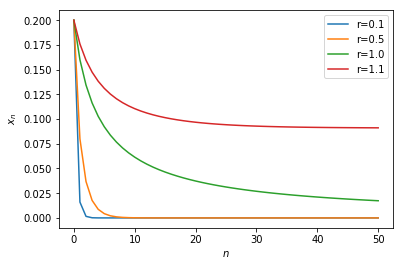
\includegraphics[scale=0.8]{Figures/rle1.png}
	\caption[An Electron]{$x_n$ vs $n$. We see that for $r<1$, $x_n$ goes to zero pretty fast.}
	\label{fig:rle1}
\end{figure}

Let's take a look at how the behaviour is for values of $r>1$ (Fig. [\ref{fig:rinbetween}]). For $r=2.8$, we see that the population oscillates a bit at the start and then settles down to a steady state value. But on the other hand, for $r=3.3$, the population just keeps oscillating periodically around the steady state value forever. This is where the logistic map becomes an important topic of study. One should note that the period of oscillations in rough $n=2$. 
\begin{figure}[h!]
	\centering
	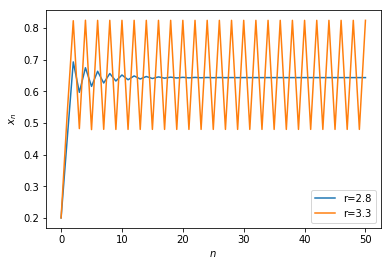
\includegraphics[scale=0.8]{Figures/rinbetween.png}
	\caption[An Electron]{$x_n$ vs $n$. For $r=2.8$, $x_n$ settles to a steady state value. For $r=3.3$, $x_n$ oscillates about the steady state.}
	\label{fig:rinbetween}
\end{figure}

Things really start getting interesting after $r=3.3$. For example, take a look at Fig. [\ref{fig:r38}], which plots the $x_n$ for $r=3.8$. We see that like $r=3.3$, $x_n$ oscillates around the steady state value, but now the period is not $n=2$! The period has now changed to a higher value. We could conjecture that for some value of the growth parameter, the period would really tend to infinity. This is a clear sign of chaos!

This is a really deep feature of the logistic map, which we shall hope to investigate further in this thesis, among other things.
\begin{figure}[h!]
	\centering
	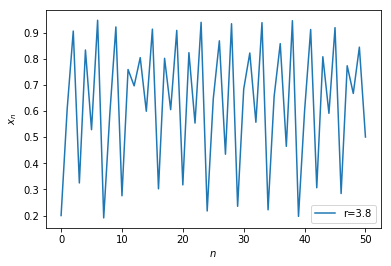
\includegraphics[scale=0.8]{Figures/r38.png}
	\caption[An Electron]{Numerical solutions for different initial conditions. Trajectories start to visibly diverge roughly around $t=30$.}
	\label{fig:r38}
\end{figure}
%\input{Chapters/Chapter5}
%% Chapter Template

\chapter{A Bound on Chaos} % Main chapter title

\label{Chapter6} % Change X to a consecutive number; for referencing this chapter elsewhere, use \ref{ChapterX}

\lhead{Chapter 6. \emph{A Bound on Chaos}} % Change X to a consecutive number; this is for the header on each page - perhaps a shortened title

Recall how we diagnose chaos in classical systems. For a dynamical variable q, we say that the system is chaotic if :- $$\frac{\partial q}{\partial q_0} = \{q(t),p_0 \} \sim e^{\lambda t},$$ where $q_0$ and $p_0$ are the initial conditions.

But in quantum mechanics, our dynamical variable is the wavefunction $\psi(x)4$, which respects unitary evolution. Due to this the inner product of the wavefunction will always have the same norm.

On thinking a bit more, one can easily see what's wrong with this analysis. We should ideally compare our wavefunction with not with the individual dynamical variables, but the phase space distribution $\rho(q,p)$.

Let us work for the moment with a spin system with spin centers $S_1, \ldots S_N$. At $t=0$, we have $[S_i,S_j]=0$. The system can be time-evolved using a Hamiltonian $H$, which we consider to be $k$-local and built out of these spin operators.


In quantum mechanics, we can use the following object for our investigations of chaos $$[W(t),V(0)]^2,$$ where 


%\input{Chapters/Chapter7}

%-------------------------------------------------------------------------------
%	THESIS CONTENT - APPENDICES
%-------------------------------------------------------------------------------

\addtocontents{toc}{\vspace{2em}} % Add a gap in the Contents, for aesthetics

\appendix % Cue to tell LaTeX that the following 'chapters' are Appendices

% Include the appendices of the thesis as separate files from the Appendices
% folder
% Uncomment the lines as you write the Appendices

%% Appendix A

\chapter{Appendix Title Here} % Main appendix title

\label{AppendixA} % For referencing this appendix elsewhere, use \ref{AppendixA}

\lhead{Appendix A. \emph{Appendix Title Here}} % This is for the header on each page - perhaps a shortened title

Write your Appendix content here.
%\input{Appendices/AppendixB}
%\input{Appendices/AppendixC}

\addtocontents{toc}{\vspace{2em}} % Add a gap in the Contents, for aesthetics

\backmatter

%-------------------------------------------------------------------------------
%	BIBLIOGRAPHY
%-------------------------------------------------------------------------------

\label{Bibliography}

\lhead{\emph{Bibliography}} % Change the page header to say "Bibliography"

\printbibliography

\end{document}
